\documentclass{article}
\usepackage{graphicx, nips} % Required for inserting images

\title{Assignment Report: Title}
\author{Student ID}

\begin{document}
\maketitle

In this report, when citing a reference, such as the xv6-book, feel free to use footnotes\footnote{Reference: https://pdos.csail.mit.edu/6.828/2005/readings/pdp11-40.pdf}.

Your report should follow the template with the following section structure.

\textbf{No page limitation}

\section{Introduction [3']}

In the introduction section, you are required to include the following:
\begin{enumerate}
    \item Provide a simple overview of how the system works when facing an mmap request.
    \item Briefly introduce what you have accomplished in this assignment.
    \item Describe any difficulties you encountered during this assignment. (If none, simply state that your progress was smooth.)
\end{enumerate}

\section{Implementation [5']}

In this section, you should present your design. For each \textbf{TODO} task, explain your implementation in a separate subsection.

It is suggested to include progress flowcharts (at most one for each subsection should suffice), like Figure~\ref{fig:sample_progress}, with text explanations.

You do not need to provide figures for \textbf{mmap} and \textbf{VMA,} as \textbf{VMA} is just a structure definition, and we have already provided the \textbf{mmap} flowchart in the instructions.

We recommend providing a succinct flowchart with a clear description if you have concerns about plagiarism detection. This flowchart should be concise and effectively illustrate your implementation without the need to copy your code directly into the report.

\begin{figure}[h]
    % \centering
    \begin{center}
    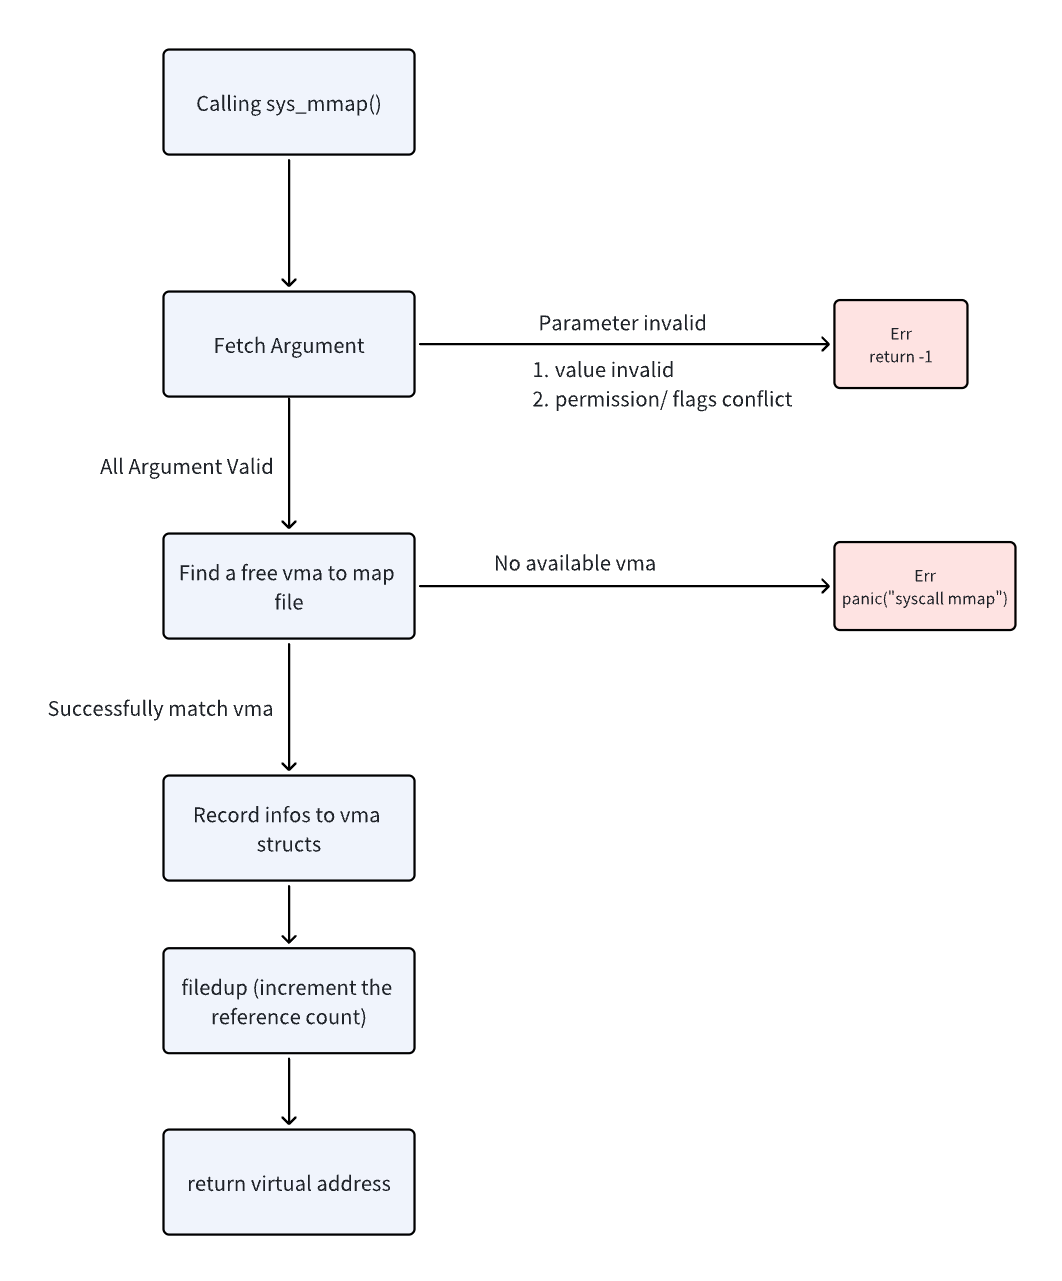
\includegraphics[width=0.4\linewidth]{sample_progress.png}
    \caption{\label{fig:sample_progress} Do NOT use this figure directly.}
    \end{center}
\end{figure}

\subsection{VMA}
\subsection{mmap}
\subsection{PageFault}
\subsection{munmap}
\subsection{Bonus}

\section{Test [2']}

Briefly discuss which part of your implementation helped you pass each test. (Several sentences for each subsection should suffice.)

\subsection{mmap f}
\subsection{mmap private}
\subsection{mmap read-only}
\subsection{mmap read/write}
\subsection{mmap dirty}
\subsection{mmap two files}
\end{document}
